% ============================ Enrico Ribiani 16-03-2021 ====================================================================
% Base per i documenti  
\documentclass{article}
% ------------ pacchetti necessari ----------------
\usepackage[a4paper, total={6in, 8in},margin=1in]{geometry} % formattazione decente della pagina
\usepackage{graphicx}                            % need for figure
\usepackage{amsmath}
\usepackage{amsfonts}                            % if you want the fonts
\usepackage{amssymb}                             % if you want extra symbols
\usepackage{graphicx}                            % need for figures
\usepackage{mathptmx}
\usepackage{float}                               % serve per mettere tabelle e immagini dove si vuole 
\usepackage[utf8]{inputenc}
\usepackage{textcomp}
\usepackage[hang,flushmargin,bottom]{footmisc}   % footnote format
\usepackage{fancyhdr, lastpage}
\usepackage{titlesec}
\usepackage[table,dvipsnames]{xcolor}
\pagestyle{fancy}
\renewcommand{\headrulewidth}{0pt}
\renewcommand*\contentsname{Indice}
\titleformat{\section}{\normalsize\bfseries}{\thesection.}{1em}{}	% required for heading numbering style
\titleformat*{\section}{\Large\bfseries}
\titleformat*{\subsection}{\large\bfseries}
\usepackage{tikz}
\usetikzlibrary{arrows,shapes,positioning,shadows,trees}

\tikzset{
  basic/.style  = {draw, text width=2cm, drop shadow, font=\sffamily, rectangle},
  root/.style   = {basic, rounded corners=2pt, thin, align=center,
                   fill=orange!70},
  level 2/.style = {basic, rounded corners=6pt, thin,align=center, fill=orange!50,
                   text width=8em},
  level 3/.style = {basic, thin, align=left, fill=orange!20, text width=6.5em}
}
%===================links=================
\usepackage{hyperref}
\hypersetup{
    colorlinks=true,
    linkcolor=Sepia,
    filecolor=magenta,      
    urlcolor=Cyan,
    pdftitle={Arduino Shield},
    pdfpagemode=FullScreen,
    }
%===================inizio pagina del titolo=================
\begin{document}
    \begin{titlepage}
\begin{flushleft}
\begin{figure}[h]
    \centering
    
\includegraphics[scale=0.8]{/home/rib/varie/logo.png}
\end{figure}
\vspace{2\baselineskip}
\Huge{\textbf{Progetto scheda di interfaccia per Arduino}}
\vfill
\LARGE Enrico Ribiani\\
\LARGE 3AUB\\
\vfill
\huge{ITT M. BUONARROTI }

%=============== fine pagina titolo ===============
\end{flushleft}
\end{titlepage}
%=============== Intestazione ===============
\pagestyle{fancy}
\fancyhead{}
\fancyhead[RO,LE]{Enrico Ribiani}
\fancyhead[LO,RE]{3AUB}
\cfoot{\thepage}
%=============== fine Intestazione ===============
\tableofcontents
\pagenumbering{arabic}
\vskip 3cm
% =============== Introduzione Generale ===============
\section{Introduzione Generale}
Questa relazione tecnica ha come obiettivo quello di redarre ciò che è stata la produzione e la progettazione della scheda 
Arduino sviluppata dalla classe \textit{3AUB} dell'istituto \href{https://www.buonarroti.tn.it/}{Buonarroti}.\\
Il progetto è stato svolto nelle ore laboratoriali di Sistemi Automatici e TPSE dopo aver completato una parte di teoria.\\
La scheda è stata realizzata principalmente per scopi didattici, per imparare come si progetta un pcb e soprattutto come si documenta la progettazione, questa parte verrà svolta
nelle prossime sezioni di questo documento.\\
% =============== Uso della scheda e specifiche di progetto ===============
\section{Uso della scheda e specifiche di progetto}
La scheda funge come shield per \textit{Arduino Uno} in quanto il sui scopo è quello di aggiungere input e output alla scheda, soprattutto 
a voltaggi come 9 e 24V, tensioni molto utilizzate in campo più industriale.\\
Quindi le morsettiere sono state progettate per essere compatibili con la scheda dal punto di vista elettrico, logico e logistico, infatti la cosa principale è che 
ci sia corrispondenza tra i pin che vengono usati per interfacciarsi e comunicare dalla scheda allo shield.

\subsection{Normative di progetto}
Sono state seguite per l'aspetto progettuale le norme \href{https://my.ceinorme.it/home.html}{CEI} riguardanti il disegno tecnico
% =============== Strumenti utilizzati ===============
\section{Strumenti utilizzati}
\subsection{Materiale di supporto}
\subsection{Software}
Abbiamo usato \textit{Multisim}[\ref{multisim}] per la seconda parte di progettazione, appunto quella che riguarda l'inizio della concretizzazione
degli schemi elettrici.\\
Infatti con questo software si opera sullo stadio precedente alla progettazione del pcb, si va soprattutto a stabilire i componenti e a scegliere i vari componenti virtuali
in base alla loro piedinatura e spazio occupato, in questa fase vengono anche implemantati i collegamenti ideali tra i vari componenti che poi verranno implementati sotto forma di piste. 
% =============== Progettazione, scelta componenti e dimensionamento ===============
\section{Progettazione, scelta componenti e dimensionamento}
La parte di progettazione iniziale della scheda, ossia quella teorica dove si vanno a trovare idealmente i componenti che andranno a comporre la scheda è stata svolta dai professori,
Per dimensionare l'aletta di raffreddamento \textit{Codice aletta} è stata usata la formula:

\begin{center}
$R_{s-a}=\frac{(Tmax-Ta)}{Pd-R_{c-s}-R_{j-c}}$\\
\end{center}
Dove \textit{$R_{c-s}$} è la R termica tra case e disspatore, \textit{$R_{j-c}$} è la R termica tra chip e case,\\ \textit{$R_{s-a}$} è la R termica tra dissipatore e ambiente.\\
\subsection{Struttura della scheda}
\begin{figure}[!h]
    \begin{center}
        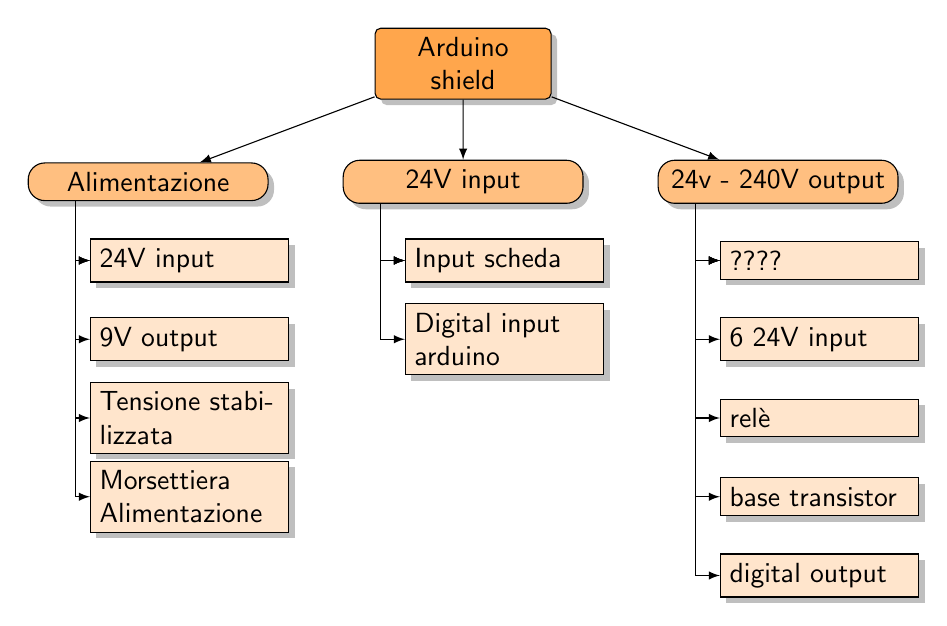
\begin{tikzpicture}[
            level 1/.style={sibling distance=40mm},
            edge from parent/.style={->,draw},
            >=latex]
          
          % root of the the initial tree, level 1
          \node[root] {Arduino shield}
          % The first level, as children of the initial tree
            child {node[level 2] (c1) {Alimentazione}}
            child {node[level 2] (c2) {24V input}}
            child {node[level 2] (c3) {24v - 240V output}};
          
          % The second level, relatively positioned nodes
          \begin{scope}[every node/.style={level 3}]
          \node [below of = c1, xshift=15pt] (c11) {24V input};
          \node [below of = c11] (c12) {9V output};
          \node [below of = c12] (c13) {Tensione stabilizzata};
          \node [below of = c13] (c14) {Morsettiera Alimentazione};
          
          \node [below of = c2, xshift=15pt] (c21) {Input scheda};
          \node [below of = c21] (c22) {Digital input arduino};
          
          
          \node [below of = c3, xshift=15pt] (c31) {????};
          \node [below of = c31] (c32) {6 24V input};
          \node [below of = c32] (c33) {relè};
          \node [below of = c33] (c34) {base transistor};
          \node [below of = c34] (c35) {digital output};
          \end{scope}
          
          % lines from each level 1 node to every one of its "children"
          \foreach \value in {1,2,3}
            \draw[->] (c1.195) |- (c11);
            \draw[->] (c1.195) |- (c12);
            \draw[->] (c1.195) |- (c13);
            \draw[->] (c1.195) |- (c14);
          
          \foreach \value in {1,...,4}
            \draw[->] (c2.195) |- (c21);
            \draw[->] (c2.195) |- (c22);
          
          \foreach \value in {1,...,5}
            \draw[->] (c3.195) |- (c31);
            \draw[->] (c3.195) |- (c32);
            \draw[->] (c3.195) |- (c33);
            \draw[->] (c3.195) |- (c34);
            \draw[->] (c3.195) |- (c35);
          
          
          \end{tikzpicture}
    \end{center}
\end{figure}
% =============== allegati ===============
\section{allegati} 
\pagenumbering{Roman}

\paragraph{Schema progetto}
\href{https://drive.google.com/file/d/1qK_MUvGxWjfc9fLc7l3a6s5mL5L6D6fg/view?usp=sharing}{Link pdf}
\begin{figure}[H]
   \centering
        \includegraphics[scale=0.5]{/home/rib/varie/progetto-ini.pdf}
       \label{prog}
       \caption{Schema iniziale per la progettazione della scheda}
\end{figure}

\paragraph{Schema di multisim}
\href{https://drive.google.com/file/d/1VOPnspiu-4T2ZOR6uaUWNH1DUEd0fUcg/view?usp=sharing}{Link immagine}
\begin{figure}[H]
   \centering
        \includegraphics[scale=0.5]{/home/rib/varie/multisimp-nobkg.png}
       \label{multisim}
       \caption{Schema Multisim con collegamenti fatti}
\end{figure}

\paragraph{Schema di Ultiboard}
\href{https://drive.google.com/file/d/1ZlJ_AIXvgzdlvAawX5noBu48i03zm5dP/view?usp=sharing}{Link immagine}
\begin{figure}[H]
    \centering
        \includegraphics[scale=0.3]{/home/rib/varie/image.png}
        \label{ultiabroad}
        \caption{Schema Ultiboard per la realizzazione del pcb}
\end{figure}

\paragraph{Render 3d}
\href{https://drive.google.com/file/d/1EMIzjUSU50ij58dLTjCctJGQM4YIgIii/view?usp=sharing}{Link immagine}
%\begin{figure}[H]
 %   \centering
  %      \includegraphics[scale=0.5]{/home/rib/varie/3dboard.png}
   %     \label{3d}
%\end{figure}
\subsection{Preventivo componenti}
% ======================================== Tabella ========================================    
    \begin{center}
        \begin{tabular}{| c | c | c | c| c |c|} 
        \hline
        \rowcolor{BurntOrange} Codice prodotto & Dispositivo & Descrizione & Quantità & Prezzo & Totale\\ [0.5ex] 
        \hline
        \rowcolor{Peach} prova & prova & prova & 8 & 8.88 & 64\\
        \hline
        \rowcolor{Apricot} prova & prova & prova & 8 & 8.88 & 64\\
        \hline
        \rowcolor{Peach} prova & prova &  prova & 8 & 8.88 & 64\\
        \hline
        \rowcolor{Apricot}prova & prova & prova & 8 & 8.88 & 64\\
        \hline
        \rowcolor{Peach} prova & prova & prova & 8 & 8.88 & 64\\
        \hline
        \rowcolor{Apricot} prova & prova & prova & 8 & 8.88 & 64\\
        \hline
   \end{tabular}
   \vskip 2mm
   \begin{tabular}[h]{|c|c|}
       \hline
        \rowcolor{BurntOrange} Prezzo totale & 121321\\
       \hline
   \end{tabular}
   \end{center}
%======================================== Fine Tabella ========================================
   \section{Bibliografia}
   \begin{itemize}
       \item \href{https://datasheetspdf.com/pdf/766811/ThinkiSemiconductor/LM78XX/1}{LM78 datasheet}
   \end{itemize}
\end{document}
